\documentclass{article}

\usepackage{times}
\usepackage{amsmath} 
\usepackage{latexsym} 
\usepackage{ dsfont }
\usepackage[usenames,dvipsnames]{xcolor}
\usepackage{tikz}
\usepackage{tikz-qtree}
\usetikzlibrary{bayesnet}
\usetikzlibrary{arrows,automata, positioning, patterns,backgrounds}


\newtheorem{definition}{Definition}
\DeclareMathOperator*{\argmax}{argmax} 
\DeclareMathOperator*{\argmin}{argmin} 
\newcommand{\E}{\mathrm{E}}

\title{Second Year Academic Committee Meeting Proposal}

\author{Eyal Dechter}

\begin{document}
\maketitle
\date

\section{Introduction}

Many of the problems an intelligent should be able to solve have
solutions that look like programs. They are hierarchical and
compositional, they reuse modular subcomponents, and they involve
higher order transformations. But the space of programs in any
langauge is vast and does not have the kind of smooth topology of
which many learning algorithms take advantage. How can intelligent
agents learn to induce programs to solve problems from experience? 

In recent work, we have proposed an algorithm for bootstrap learning
of modular concepts to facilitate program induction. This algorithm,
which we call E.C. (for Exploration-Compression), iteratively learns a
library of program primtives that enable the algorithm to explore the
space of relevant solutions more efficiently. In the first step of
each iteration, E.C. searchs (\textbf{explores}) the space of ``short''
programs given the current library for programs that solve the tasks
at hand. In the second step, E.C finds common subroutines in the
successful programs and uses these to construct a new library of
program primitives (\textbf{compression}).

In our work on this algorithm, we found this simple procedure can
quickly make search over the space of programs much more
efficient. Whereas the algorithm finds solutions to almost no programs
in the initial iterations, it quickly finds a set of program
primitives that allows it to traverse the set of relevant programs
much more effectively.

I propose to continue on the research program initiated by this
work. In the remainder of this document, I will detail my ideas for
current and future research in this area.

\section{The E.C.E.M algorithm}

The E.C. algorithm, as presented so far, draws on many ideas in
machine learning; these include Learning To Learn, Minimum Description
Length, and Predicate Invention in Inductive Logic
Programming. However, we aim to show that the E.C. algorithm, or
something very similar to it, can be derived as the application of E.M
to MAP inference for a generative model in which a latent stochastic
grammar (nature) generates programs. Individual tasks are the ``data''
of this generative process, for the rewards they provide convey
how close a particular solution is to the task the nature had in
mind. This generative process is depicted in Figure~\ref{fig:ECGM}.
\begin{figure}
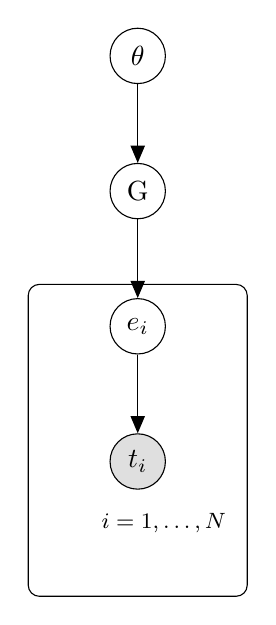
\begin{tikzpicture}[->, circle]

\node[latent] (theta) {$\theta$} ;
\node[latent, below=of theta] (G) {G} ;
\node[latent, below=of G]     (e) {$e_i$} ;
\node[obs, below=of e]     (t) {$t_i$} ;

\edge {theta} {G};
\edge {G} {e};
\edge {e} {t};

\plate {plate} {
  (e)(t)}{$i=1, \dots, N$};

\end{tikzpicture}
\caption{Generative model of program induction
  tasks. \label{fig:ECGM}}
\end{figure}

of E.C as finding the grammar $G$ that maximizes the maximizes the
posterior probability of $G$ given the tasks and the prior on the
grammar. We can use E.M. to solve
this procedure. We can derive the E.M update rule as follows: 

\begin{align}
G_{new} &= \argmax_{G'} 
     \E [\log \prod_i p(t_i, e_i | G') | G, t_1, \dots, t_N]\\
        =& \argmax_{G'} \E 
           [\sum_i^N \log p(t_i, e_i | G') | G, t_1, \dots, t_N]\\
  =& \argmax_{G'} \sum_i^N \E [\log p(t_i |  e_i) | G, t_1, \dots, t_N] + 
  \sum_i^N \E [\log p(e_i |  G') | G, t_1, \dots, t_N]\\
  =& \argmax_{G'}  
  \sum_i^N \E [\log p(e_i |  G') | G, t_1, \dots, t_N]\\
  =& \argmax_{G'} \sum_i^N \E [\log p(e_i |  G') | G, t_1, \dots, t_N]\\
  =& \argmax_{G'} \sum_i^N \sum_{e_j \sim p(e|G)}
                            p(t_i | e_j, G) 
                            \log p(e_i |  G')
\end{align}

Part of the E.M. algorithm applied to this problem
requires taking the expectation of a function with respect to the
probability of a program given the current grammar and the tasks. This
expectation can be approximated by by likelihood reweighted sampling,
in which we sample programs from the prior and weight by their fit to
the task. This is very similar to the exploration step of the
E.C. algorithm. 

Once we estimated this expectation using likelihood reweighted
sampling, we still need to perform the optimization of the objective
over grammars. Any prior distribution over grammars which favors a
short description length is going to support populating the grammar
with production rules corresponding to frequently occuring
subroutines. Thus, the maximization of the object involves a
compression-like step.

Thus, we see that we arrive at an iterative procedure that
successively re-estimate the latent grammar in much the same way that
the E.C. algorithm does. 

\section{E.C. with partial solutions}

One of key limitations of the E.C. algorithm as presented so far is
that it does not enable the problem solving agent to utilize
information about partial solutions. But humans, especially when they
are learning to perform a task, rely on incremental feedback from the
world. Thus, if there is a way to partially evaluate solutions, we
would like to find a way to incorporate this into our learning
algorithm. 

We are currently developing an algorithm that would do just this. To
make our approach concrete, suppose your task is to build a structure
of blocks that reaches a specified height but is both stable and uses
as few blocks as possible. Moreover, in every task the space has
different obstacles present and perhaps different building blocks
available.

A solution to this problem can be represented as a list of block
placing actions. We could ask our learning agent to produce a program
that generates a list of such actions. Instead, however, we will ask
the agent to generate a program which transform one list of actions
to another. These can be arbitrary transformations. For example, a
transformation can append a new action to the list of actions, it can
repeat the current list of actions a fixed number of times, it can
reverse the list of actions, and it can shift every action in the list
over by some vector. 

For each task, the agent starts with an empty list of actions and
searches for a sequences of such transformations whose composition
solve the given task. Every time the agent performs such a
transformation, it can calculate the difference between the objective
function before the transformation and the object function before;
this provides some information about the utility of that particular
transformation.

We are currently working on implementing this approach both in the
domain of tower building and in the domain of constructive solid
geometry. In the latter domain, the task is to discover the set of 3D
object transformations that can reconstruct an input solid. 

\section{Looking head}
Not only can humans score partial solutions to estimate their
efficacies, but they can also plan future actions by taking the
current state into account. That is, humans can look at the world,
analyze it, and use that analysis to choose their next step. The
algorithm we proposed in the previous section does not do this. It
only takes into account the previous actions, not the resulting world
state. 

Eventually, then, we would like to take sensory information as an
input this program induction system. The major unanswered question is
what the form of the sensory information should be? If its visual
information, can we really expect our program induction system to
learn to extract useful information from an image via trial and error?
If not, then what is the alternative?

\end{document}
